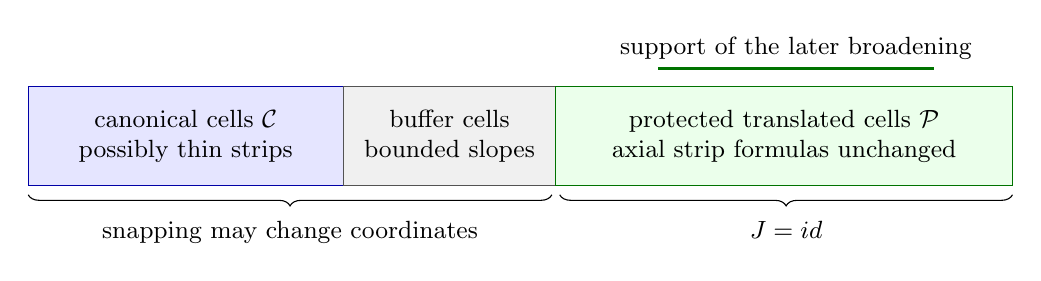
\begin{tikzpicture}[x=1cm,y=1cm,font=\small]
\filldraw[fill=blue!10,draw=blue!65!black] (0,0) rectangle (4,1.25);
\filldraw[fill=gray!12,draw=gray!65!black] (4,0) rectangle (6.7,1.25);
\filldraw[fill=green!8,draw=green!45!black] (6.7,0) rectangle (12.5,1.25);
\node[align=center,text width=3.7cm] at (2,.625)
  {canonical cells $\mathcal C$\\possibly thin strips};
\node[align=center,text width=2.4cm] at (5.35,.625)
  {buffer cells\\bounded slopes};
\node[align=center,text width=5.5cm] at (9.6,.625)
  {protected translated cells $\mathcal P$\\axial strip formulas unchanged};
\draw[decorate,decoration={brace,mirror,amplitude=4pt}]
  (0,-.12) -- (6.65,-.12)
  node[midway,below=6pt,align=center] {snapping may change coordinates};
\draw[decorate,decoration={brace,mirror,amplitude=4pt}]
  (6.75,-.12) -- (12.5,-.12)
  node[midway,below=6pt] {$J=\operatorname{id}$};
\draw[very thick,green!45!black] (8,1.48) -- (11.5,1.48);
\node[above,align=center] at (9.75,1.48)
  {support of the later broadening};
\end{tikzpicture}